\documentclass[11pt, A4paper,norsk]{article}
\usepackage[utf8]{inputenc}
\usepackage[T1]{fontenc}
\usepackage{babel}
\usepackage{amsmath}
\usepackage{amsfonts}
\usepackage{amsthm}
\usepackage{amssymb}
\usepackage[colorlinks]{hyperref}
\usepackage{listings}
\usepackage{color}
\usepackage{hyperref}
\usepackage{graphicx}
\usepackage{cite}
\usepackage{textcomp}

\definecolor{dkgreen}{rgb}{0,0.6,0}
\definecolor{gray}{rgb}{0.5,0.5,0.5}
\definecolor{daynineyellow}{rgb}{1.0,0.655,0.102}
\definecolor{url}{rgb}{0.1,0.1,0.4}

\lstset{frame=tb,
	language=Python,
	aboveskip=3mm,
	belowskip=3mm,
	showstringspaces=false,
	columns=flexible,
	basicstyle={\small\ttfamily},
	numbers=none,
	numberstyle=\tiny\color{gray},
	keywordstyle=\color{blue},
	commentstyle=\color{daynineyellow},
	stringstyle=\color{dkgreen},
	breaklines=true,
	breakatwhitespace=true,
	tabsize=3
}

\lstset{inputpath="C:/Users/Torstein/Documents/UiO/Fys2140/Python programmer"}
\graphicspath{{C:/Users/Torstein/Documents/UiO/Fys2140/"Python programmer"/}}
\hypersetup{colorlinks, urlcolor=url}

\author{Torstein Solheim Ølberg}
\title{Svar på Oblig nr. 3 i Fys2140}



%\lstinputlisting{Filnavn! type kodefil}
%\includegraphics[width=12.6cm,height=8cm]{Filnavn! type png}



\begin{document}
\maketitle
	\begin{center}
\Large \textbf{Oppgaver}
	\end{center}









		\paragraph{1.}
			\subparagraph{a)}
				\begin{flushleft}
De Broglie bølgelengden er gitt ved utrykket $\lambda = \frac{h}{p}$, og for relativistiske hastigheter er $p = \sqrt{\frac{E^2 - m_0^2c^4}{c^2}}$. Da har vi at $\lambda = \frac{h}{\sqrt{\frac{E^2 - m_0^2c^4}{c^2}}}$. Når vi vet at $E_{tot} = E_h + E_k = m_0 c^2 + e V$, hvor $E_k$ er den kinetiske energien til en partikkel som den har fått av å bli akselerert i et elektrisk felt med potensial $V$, så blir $\lambda = \frac{h}{\sqrt{\frac{(m_0 c^2 + eV)^2 - m_0^2c^4}{c^2}}}$
				\end{flushleft}
				\begin{gather*}
\lambda = \frac{h}{\sqrt{\frac{(m_0 c^2 + eV)^2 - m_0^2c^4}{c^2}}} = \frac{h}{\sqrt{\frac{2 m_0 c^2 e V + e^2 V^2}{c^2}}} \\
\lambda = \frac{h}{\sqrt{2 m_0 e V + \frac{(eV)^2}{c^2}}} = \frac{h}{\sqrt{2m_0 e V + (2m_0 e V)\frac{e V}{2 m_0 c^2}}} \\
\lambda = \frac{h}{\sqrt{2m_0 e V} \sqrt{ 1 + \frac{e V}{2 m_0 c^2}}} = \frac{h}{\sqrt{2m_0 e V}} \left( 1 + \frac{e V}{2 m_0 c^2} \right)^{- \frac{1}{2}}
				\end{gather*}








			\subparagraph{b)}
				\begin{flushleft}
I den ikke-relativistiske grensen er hastigheten til partikkelen så lav at du kan bruke vanlig ikke-relativistisk bevegelsesmengde, og utrykket for $\lambda$ blir $$\lambda = \frac{h}{p} = \frac{h}{m_0 v}$$
				\end{flushleft}









			\subparagraph{c)}
				\begin{gather*}
\gamma = \frac{1}{\sqrt{1 - \frac{v^2}{c^2}}} = \frac{c}{\sqrt{c^2 - v^2}} = \frac{\sqrt{v^2}}{\beta \sqrt{c^2 - v^2}} = \frac{1}{\beta} \sqrt{\frac{1}{\frac{1}{\beta}^2 - 1}} = \frac{1}{\sqrt{1 - \beta^2}} \\
\lambda = \frac{h}{p} = \frac{h}{\gamma m_0 v} = \frac{h}{\frac{E_0 v}{c^2}} \cdot \sqrt{1 - \beta^2} = \frac{h}{\frac{E_0}{c}} \cdot \frac{\sqrt{1 - \beta^2}}{\beta} \\
\lambda = \frac{h c}{E_0} \cdot \frac{\sqrt{1 - \beta^2}}{\beta} = \frac{1240 MeV fm}{E_0} \cdot \frac{\sqrt{1 - \beta^2}}{\beta} \\
\lambda = \frac{1.24 \cdot 10^{-2}}{E_0 (MeV)} \cdot \frac{\sqrt{1 - \beta^2}}{\beta} \text{Å}
				\end{gather*}
			









		\paragraph{2.}
			\subparagraph{a)}
				\begin{flushleft}
Bruker likningene $E = \omega \hbar$, $p = \hbar k$ og $E^2 = p^2c^2 + m^2 c^4$
				\end{flushleft}
				\begin{gather*}
\omega = \frac{E}{\hbar} = \frac{\sqrt{p^2 c^2 + m^2 c^4}}{\hbar} = \sqrt{c^2 \frac{p^2}{\hbar^2} + c^2 \left(\frac{m c}{\hbar}\right)^2} \\
\omega = c \sqrt{\frac{\hbar^2 k^2}{\hbar^2} + \left( \frac{m c}{\hbar} \right)^2} = c \sqrt{k^2 + \left( \frac{m c}{\hbar} \right)^2}
				\end{gather*}










			\subparagraph{b)}
				\begin{gather*}
v_f = \frac{\omega}{k} = \frac{c \sqrt{k^2 + \left( \frac{m c}{\hbar} \right)^2}}{k} = \frac{c}{k} \sqrt{k^2 + \left( \frac{m c}{\hbar} \right)^2} \\
v_g = \frac{d \omega}{dk} = \frac{d}{dk} \left( c \sqrt{k^2 + \left( \frac{m c}{\hbar} \right)^2} \right) = c\frac{1}{2} \frac{2k}{\sqrt{k^2 + \left( \frac{m c}{\hbar} \right)^2}} = \frac{c k}{\sqrt{k^2 + \left( \frac{m c}{\hbar} \right)^2}} \\
v_f \cdot v_g = \frac{c}{k} \sqrt{k^2 + \left( \frac{m c}{\hbar} \right)^2} \cdot \frac{c k}{\sqrt{k^2 + \left( \frac{m c}{\hbar} \right)^2}} = c^2
				\end{gather*}









			\subparagraph{c)}
				\begin{flushleft}
Hvis fasehastigheten $v_f > c$, så vil det si at denne hastigheten ikke kan være hastigheten til partikkelen. Men bortsett fra det er dette fullstendig fysisk mulig. Lorentzfaktoren $$\gamma = \frac{1}{\sqrt{1 - \frac{v^2}{c^2}}}$$ sier ingen ting om at det kan finnes hastigheter over $c$, bare at en hastighet ikke kan passere $c$. $v_g$ er derimot mindre enn $c$ og kan dermed være partikkelens hastighet, noe den viser seg å være.
				\end{flushleft}









		\paragraph{3.}
			\subparagraph{a)}
				\begin{flushleft}
Velger at $t = 1$, at posisjonen er $-100 < x < 100$ og at antall posisjonssteg er $N = 10000$.
				\end{flushleft}
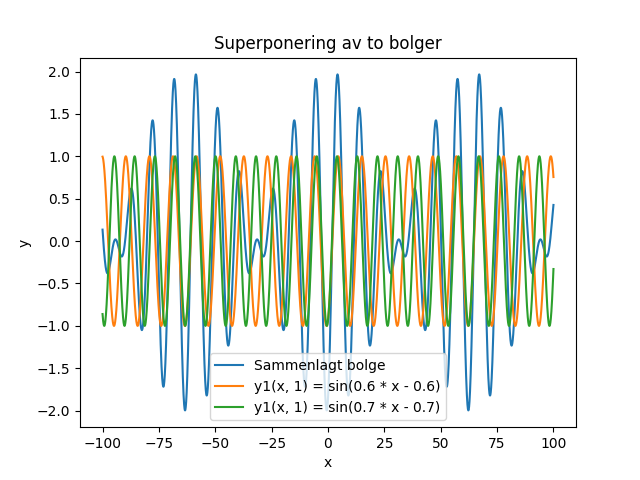
\includegraphics[width=12.6cm,height=8cm]{Figur_01.png} \\
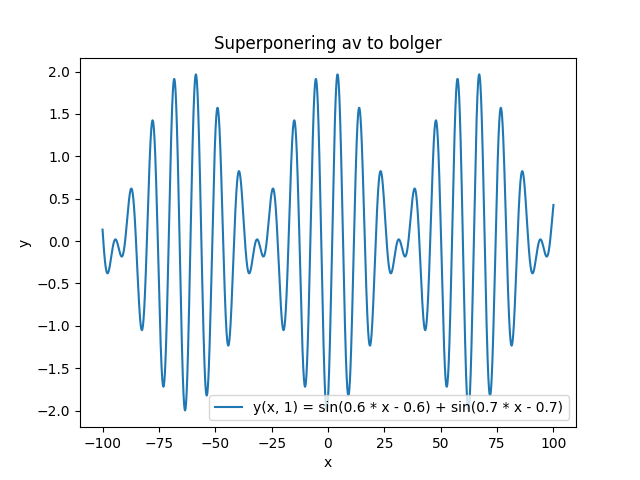
\includegraphics[width=12.6cm,height=8cm]{Figur_02.png}
\lstinputlisting{Oblig3_3a.py}








			\subparagraph{b)}
				\begin{flushleft}
$$y(x, t) = \sin\left(kx - w(k)t\right)$$
Ut i fra uttrykket $\omega(k) = c \sqrt{k^2 + \left( \frac{m c}{\hbar} \right)^2} = \sqrt{k^2 + 1}$ vil bølgen bevege seg med hastighet $v_g$ mot venstre. Når du superponerer to bølger blir det nye bølgetallet gjennomsnittet av bølgetallet til de to den er laget av. Altså $0.6 + \frac{0.7 - 0.6}{2} = 0.65$
				\end{flushleft}
				\begin{gather*}
v_f = \frac{c}{k} \sqrt{k^2 + \left( \frac{m c}{\hbar} \right)^2} = \frac{\sqrt{k^2 + 1}}{k} = 1.8349c \\
v_g = \frac{c k}{\sqrt{k^2 + \left( \frac{m c}{\hbar} \right)^2}} = \frac{k}{\sqrt{k^2 + 1}} = 0.5450c \\
				\end{gather*}











			\subparagraph{c)}
				\begin{flushleft}
Velger $a = 1$, $N = 100000$ og at $-20 < x < 20$. Resten av konstantene er de samme som tidligere.
				\end{flushleft}
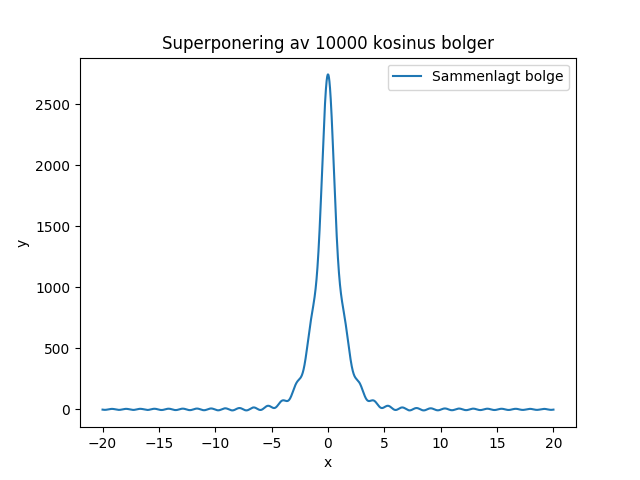
\includegraphics[width=12.6cm,height=8cm]{Figur_03.png}
\lstinputlisting{Oblig3_3c.py}
\end{document}